% !TeX spellcheck = pl_PL
\chapter{Wymagania}\label{chap:wymagania}
Aplikacja ma na celu pomóc użytkownikowi zrozumieć i zobrazować działanie algorytmów na sieciach przepływowych. Student, który przygotowuje się do kolokwium z przedmiotów związanych z algorytmiką powinien móc utworzyć własną sieć przepływową, prześledzić działanie wybranych algorytmów krok po kroku oraz móc zapisać postęp swojej pracy. Aplikacja ma mieć charakter edukacyjny, umożliwić jak najlepsze przyswojenie omawianych w pracy algorytmów. Wymagania zostały przedstawione w postaci przypadków użycia na rysunku \ref{fig:userCases}.
\begin{figure}[H]
	\centering
	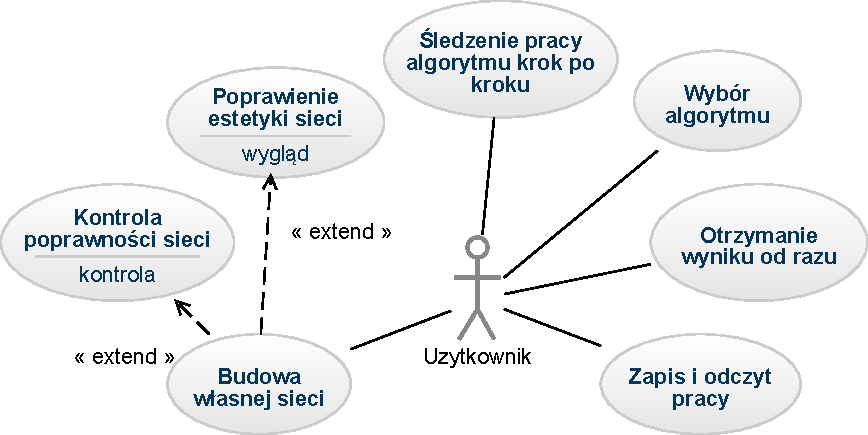
\includegraphics[width=0.8\textwidth]{./img/user_case2}
	\caption{Funkcjonalności wymagane przez potencjalnego użytkownika}
	\label{fig:userCases}
\end{figure}
Ponadto aplikacja powinna zapewnić niezawodność wykonywanych algorytmów. Jeżeli sieci zbudowane przez użytkownika są niepoprawne i nie spełniają założeń, nie powinno dać się wykonywać algorytmów. Użytkownik powinien zostać poinformowany jakie dokładnie błędy popełnił w budowie i co należy zrobić by je wyeliminować. Jeżeli siec jest poprawna, algorytm powinien móc dać się wykonać, a jego proces być łatwo kontrolowany przez użytkownika, najlepiej przy pomocy kilku przycisków. Wszystkie zmiany, jakie wprowadził algorytm w danym kroku powinny zostać opisane oraz podświetlone na grafie podglądowym, jeżeli jest to możliwe. Algorytmy wyznaczania maksymalnego przepływu, opisane w rozdziale \ref{ch:analiza}, tworzą struktury pośrednie i operują na nich, aplikacja powinna również zapewnić możliwość śledzenia wszystkich działań wykonanych na nich.\\\indent
Czas oczekiwania na wykonanie pojedynczego kroku algorytmu powinien być krótki, nieprzekraczający kilku sekund, aby nie nadużywać cierpliwości użytkownika. Aplikacja powinna umożliwiać śledzenie pracy algorytmu zarówno przez małe kroki, jak i skok do końca działania procesu i otrzymania wyniku natychmiastowo, np. w celu porównania go z obliczeniami na kartce.